\title{Approximation for Piecewise Linear Functions}
 
\section*{Introduction}
For many continuous probabilistic planning problems it is useful to describe transition or reward functions as piecewise linear functions of problem variables. This class of functions can be represented efficiently in linear eXtended Algebraic Decision Diagrams (LinXADDs). However, as the complexity of the function grows, the number of different cases and linear pieces may become intractably large even with few variables. A practical approach to tackle larger problems is to make approximations with a limited error, reducing the number of cases and of different linear functions. Our goal here is to describe an efficient method for obtaining the best linear approximation, and the error incurred, for two distinct linear functions defined on cases.

\section{Problem and Solution} 
\label{probSol} 
A better definition of our mathematical objects is in appendix \ref{appA}. For approximately representing complex piecewise linear functions it is helpful to determine if the number of cases and linear functions can be reduced, thus we intend to replace two case functions with a single case function. More formally, given two case linear functions $L_1 = ( f_1, \phi_1 )$ and $L_2 = ( f_2, \phi_2 )$, our goal is to determine a case linear function $L^* = (f^*,\phi_1 \cup  \phi_2)$ that minimizes the incurred  error:
$$ E(f) = \max ( |f - f_1|_{\phi_1} , |f - f_2|_{\phi_2} )$$
$$f^* = argmin_f E(f) $$
This optimization problem is complex because we have maximization and minimization on different variables, and a maximum in the objective function.
In order to solve it an iterative constraint generation based algorithm is proposed. Basically, for the minimization step, we will relax the maximum error on $\phi_1 \cup \phi_2$ to be the maximum error on a finite set of points, which become a finite set of constraints.  Using the solution for this relaxed problem we solve the maximization to find greatest error points in the region and then include this points as new constraints in the minimization. After a finite number of iterations the solution will no longer be improving (the maximum error points will already be included in the constrains) and the algorithm has converged to the true best approximation.

\section{Algorithm}
We will define an iterative algorithm using linear solvers in two different steps. Algorithm \ref{alg:glo} is the main method that solves the approximation problem using the functions $MAX\_ERROR$ and $BEST\_APPROX$, which use a linear programming, $LP\_Solve($ max or min$, objective, constraints)$.

\begin{algorithm}[!h]
\dontprintsemicolon
\KwIn{A pair of case linear functions $L_1 = ( f_1, \phi_1 )$ and $L_2 = ( f_2, \phi_2 ).$}
\KwOut{$L^* = (f^*,\phi_1 \cup  \phi_2)$ that best approximates $L_1$ and $L_2$.}
$f \gets 0$\;
$points \gets \emptyset$\;
$new\_points = MAX\_ERROR(f, L_1,L_2)$\;
\While{$new\_points \not \subset points$} {
	$points = points \cup new\_points$\;
	$f = BEST\_APPROX(f_1,f_2,points)$\;
	$new\_points = MAX\_ERROR(f, L_1,L_2)$\;}
\Return{$f$}\;
\caption{{\sc Constraint Generation MiniMax} finds the best case linear function}
\label{alg:glo}
\end{algorithm}

\subsection{MAX\_ERROR}
We show that for a given $f$ the internal maximization can be done with four linear optimizations:

Remembering $ |f - f_1| = max (f-f_1,f_1-f)$ we get that our error is the greater of four similar restricted maximizations.
$$ E(f) =\max \left( max_{x\in \phi_1} (f - f_1) (x),
max_{x\in \phi_1} (f _1- f) (x),
max_{x\in \phi_2} (f - f_2) (x),
max_{x\in \phi_2} (f_2 - f) (x)
\right)$$
For simplicity we will inspect one of these, considering that our functions are all linear, we can use:
$$ f = \sum_{i=0}^n w_i x_i,  \mbox{\rule{1cm}{0cm}} 
f_1 = \sum_{i=0}^n \alpha_i^1 x_i$$

$$max_{x\in \phi_1} (f _1- f) (x) = max_{x\in \phi_1}\sum_{i=0}^n (w_i- \alpha_i^1) (x) $$
which is a linear optimization problem for x, resulting in the maximum error and the solution $x^*$  where this error is maximum.
This is illustrated in algorithm \ref{alg:max}.

\begin{algorithm}[!h]
\dontprintsemicolon
\KwIn{Two case linear functions $L_1 = ( f_1, \phi_1 ), L_2 = ( f_2, \phi_2 )$ and an approximation $f$ }
\KwOut{Four points where each of the four errors is maximal.}
$p_1 \gets LP\_Solve(max _x, f-f_1,\phi_1)$\;
$p_2 \gets LP\_Solve(max_x, f_1-f,\phi_1)$\;
$p_3 \gets LP\_Solve(max_x, f-f_2,\phi_2)$\;
$p_4 \gets LP\_Solve(max_x, f_2-f,\phi_2)$\;
\Return{$\{p_1,p_2,p_3,p_4\}$}\;
\caption{{\sc MAX\_ERROR} finds the points of maximum error}
\label{alg:max}
\end{algorithm}

\subsection{BEST\_APPROX}
We show that this maximum error points induce constraints for a linear relaxation of the minimization problem.
A relaxation of the minimization problem is instead of minimizing the maximum error in all points of $\phi_1 \cup \phi_2$, minimizing the error on two finite set of points $X^1 = \{ x^1_1, ..., x^1_{m_1} \} \subset   \phi_1$ and $X^2 = \{ x^2_1, ..., x^2_{m_2} \} \subset   \phi_2$
	
$$ \tilde{E}(f) =\max \left( (f - f_1) (x^1_1), ... , (f - f_1) (x^1_{m_1}),  (f _1- f) (x^1_1), ... ,  (f - f_2) (x^2_1), ... , (f_2 - f) (x^2_{m_2})
\right)$$


$$\tilde{f} = argmin_w \tilde{E}(f) $$
or, converting the max into constraints by adding an artificial variable $Z$.

$$\tilde{f} = argmin_{f,Z}  Z $$
s.t. 
$$
	\begin{array}{llll}
		Z & \geq & (f - f_1) (x^1_j) & \mbox{for } j = 1,...m_1\\
		Z & \geq & (f_1 - f) (x^1_j) & \mbox{for } j = 1,...m_1\\
		Z & \geq & (f - f_2) (x^2_k) & \mbox{for } k = 1,...m_2\\
		Z & \geq & (f_2 - f) (x^2_k) & \mbox{for } k = 1,...m_2\\
	\end{array}
$$

This is now a linear problem in the coefficients of $f$, the solution Z is the error incurred in the approximation. This is illustrated in algorithm \ref{alg:best}.

\begin{algorithm}[!h]
\dontprintsemicolon
\KwIn{Two case linear functions $L_1 = ( f_1, \phi_1 ), L_2 = ( f_2, \phi_2 )$ and a set of $points$ where to find the best approximation for them}
\KwOut{Best linear approximation for both $f$.}
$constr \gets \emptyset$\;
\For {$p \in points$}{ 
	\If {$p \in \phi_1$}{
		$constr \gets constr \cup \{ (Z \geq (f - f_1) (p)), (Z \geq (f_1 - f) (p) )\} $}\;
	\If {$p \in \phi_2$}{
		$constr \gets constr \cup \{ (Z \geq (f - f_2) (p)), (Z \geq (f_2 - f) (p) )\} $}\;
}\;
$f \gets LP\_Solve(min_{f,Z}, Z, constr)$\;	
\Return{$f$}\;
\caption{{\sc BEST\_APPROX} finds the best approximation on points}
\label{alg:best}
\end{algorithm}

\section{Conclusion}
We have presented an iterative constraint generation method for obtaining the best case linear function for approximating two other case linear functions. The algorithm has implemented on the java XADD package, was used in small tests for pruning specific trees and will soon be tested on diagrams from solution of continuous MDPs. 
\newpage
\appendix
\section{Definitions} 
\label{appA} 

First we give the basic definitions of our mathematical model.\\
Let  $\mathbb{X}$ be a set of real valued variables: $\mathbb{X} = \{ x_1, x_2, ... , x_n\ | x_i \in \mathbb{R}, \forall i\}$\\
A linear function $f: \mathbb{R}^n \rightarrow \mathbb{R}$ over $\mathbb{X}$ is a linear combination of the variables and a constant 
$$f(x) = \sum_{i=0}^n { \alpha_i x_i}$$ where $\alpha_i \in \mathbb{R}$ and $x_0$ equals $1$.\\
A linear constraint is a region of $\mathbb{R}^n$ defined by the signal of a linear function $f$:
$$c = \{	x \in \mathbb{R}^n | f(x) \geq 0 \} $$
A linear case $\phi$ is the region defined by $m \in \mathbb{N}^+$ linear constraints $c_1, c_2, ... c_m$:
$$ \phi =c_1 \cap c_2 \cap ... \cap c_m $$

A case linear function is a pair $(f, \phi)$, where $f$ is a linear function and $\phi$ is a linear case.  $(f, \phi)$ denotes the partial function equal to $f$ in $\phi$ and undefined elsewhere.

A piecewise linear function is a function $f: \mathbb{R}^n \rightarrow \mathbb{R}$ defined by joining different case linear functions with exclusive cases:
$$ f = 
\left\{
	\begin{array}{ll}
		\phi_1 : & f_1(x)\\
		\phi_2 : & f_2(x)\\
		... & \\
		\phi_m : & f_m(x)\\
	\end{array}
\right.
$$
where $\phi_i \cap \phi_j = \emptyset$ if $i \neq j$

\section{Underconstrained Problem} 
\label{appB} 

A clear example of a function where approximation can be helpful is a regular difference step function, as the one in picture \ref{stepf}. 
\begin{figure}[!h]
\center
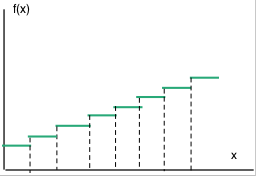
\includegraphics[scale=0.9]{Figures/step.png}
\caption{A linearizable step function.}
\label{stepf} 
\end{figure}

For this function it seems clear that with a small error, a much simpler representation can be achieved by modifying the linear function and merging the regions. We would like to represent it concisely as in figure \ref{steplin}.
\begin{figure}[h]
\center
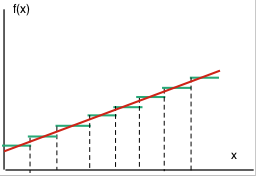
\includegraphics[scale=0.9]{Figures/steplin.png}
\caption{An approximation reducing the number of cases.}
\label{steplin} 
\end{figure}
Considering the complexity of comparing multiple functions our approach would be to compare and merge the regions pairwise, making successive merges until all regions have collapsed, in a procedure as shown in picture \ref{steplining}. While our merging algorithm minimizes the error in each merge the total error is evaluated as the sum of errors incurred in successive merges, and is not explicitly minimized.

\begin{figure}[!h]
\centering
\begin{minipage}{.7\textwidth}
  \centering
  \subfigure[Original] {
	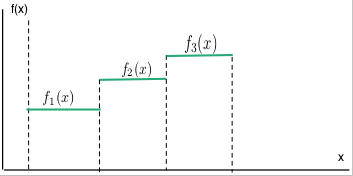
\includegraphics[scale=0.75]{Figures/step1.png}
	\label{step1}
  }
\end{minipage}
\begin{minipage}{.7\textwidth}
\centering
\subfigure[Step1] {
	 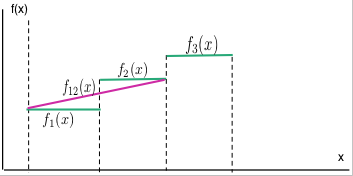
\includegraphics[scale=0.75]{Figures/step12.png}
	\label{step2} 
}
\end{minipage}
\begin{minipage}{.7\textwidth}
\centering
\subfigure[Step2]{
	 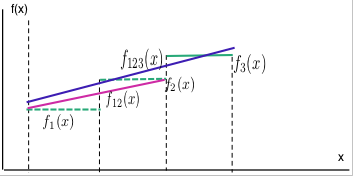
\includegraphics[scale=0.75]{Figures/step123.png}
	 \label{step2}
}
\end{minipage}
\caption{ Making the approximation by successive merging}
 \label{steplining}
\end{figure}

Therefore, while making experiments it became clear that when merging linear functions with the same angular coefficient, as the step function case, the problem of minimizing the maximal error has various solutions, out of which our algorithm will arbitrarily choose one. An example is depicted in figure \ref{steplin2}. Both functions $f_1(x)$ and $f_2(x)$ approximate the step function optimally according to the maximum error so either may be chosen by our algorithm.This reveals that the problem specified earlier, of finding the best linear case approximation for two linear case functions is possibly underspecified.  Its is suggested that since $f_2(x)$ yields a smaller average error than $f_1(x)$ it could be used to improve the approximation. Minimizing other forms of errors would avoid this underspecification. Another concern is if choosing the appropriate optimal function will lead to a better total error, as the propagations of errors for successive merges may not provide the overall best approximation.
\begin{figure}[h]
\center
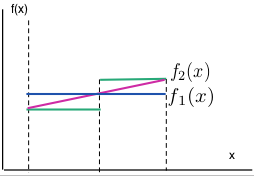
\includegraphics[scale=0.9]{Figures/step2lin.png}
\caption{Two optimal MaxError approximations.}
\label{steplin2} 
\end{figure}